The Recipe Approximation Problem (RAP) was originally conceived by Kyle Oliver
in \cite{oliver_geniusv2:_2009}. Its conception was the result of conversations
with scientists of the VISION fuel cycle simulation team \cite{vision2009}
concerning what was then called the ``Winery Problem'' due to the similarity to
the problem of mixing vintages of wine to match a given ``recipe''. This work
expands Oliver's initial formulation by correcting an error and expanding the
single-request formulation to an $n$-request formulation.

The Recipe Approximation Problem (RAP) seeks to model a separations facility
matching reactor fuel orders. Conceptually, the problem formulation is
relatively simple. The basic constituents include a set of barrels of separated
material, $B$, and a set of target recipes, $T$. Each barrel is defined by a
quantity, $m_b$, and isotopic quality vector, $I_b$. The barrel mass matrix,
$M$, is constructed of column vectors by multiplying $m_b$ and $I_b$ for each
barrel. Similarly, each target recipe is defined by a quantity, $m_t$, and
isotopic quality vector, $I_t$. A mass vector for the target recipe is defined
by multiplying $m_t$ and $I_t$. The goal of the program is to find a extraction
matrix, $X$, which minimizes the residual of some parameter associated with the
matching of recipes, where the most straight forward parameter is the target
recipe isotopic masses. Each constituent, $x_{b,t}$, represents a fraction of
barrel, $b$, taken to match a target recipe, $t$. The problem is shown
graphically in Figure \ref{fig:rap}, displaying the set of barrels, $B$, the set
of fuel requests, $R$, and the set of extraction fractions, $X$.

\begin{figure}[h]
  \begin{center}
    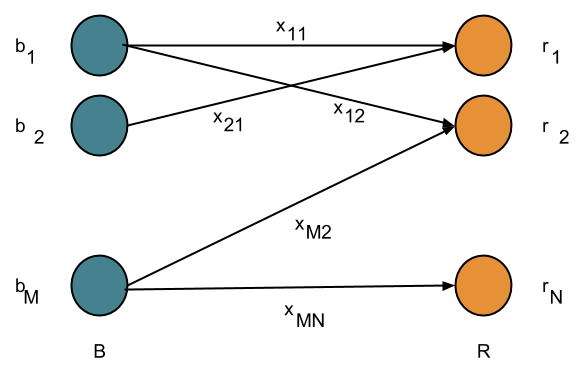
\includegraphics[width=8cm]{./chapters/research/rap.png}
  \caption{A graphical view of an example solution to the Recipe Approximation 
           Problem.}
  \label{fig:rap}
  \end{center}
\end{figure}

The optimal extraction fractions are modeled as the solution to an approximation
linear program, the foundations of which were described in
\S\ref{sec:approx}. The most straightforward formulation of the RAP is first
described, expanding upon the work in \cite{oliver_geniusv2:_2009}. The addition
of other domain-specific constraints is then described. Finally, a more abstract
version that adds a notion of agency to the problem formulation is provided.
